\chapter{Power Plant Cost Model Results}\label{ch6:cm_results}

Chapter \ref{ch4:cm_prep} outlined the cost modeling strategy for a hypothetical 5 MW expansion project of the Lightning Dock power plant in Animas Valley, NM. This chapter reviews the results of the different model approaches, explores insights gained from those models, and describes how this approach mitigates risks associated with geothermal production.

\section{Static Model}
\label{ch6:static_mod}

\subsection{Model Selection}
\label{ch6:static_select}

Section \ref{ch4:cm_rev} described the use of brine effectiveness in the cost model for determining the power output of a binary cycle plant for a given production temperature and flow rate. This formulation provides a choice of how to manage the cost model mechanics due to a trade-off between plant capacity and flow rate for a given brine effectiveness (Equation \ref{eq:cm_rev}).

In addition, installation of the Lightning Dock expansion can take place over a variety of different deployment schedules due to the modularity of the system. Rather than drill ten wells and install five binary cycle plants all at once, delaying aspects of the installation can be financially beneficial and less of an initial risk for the project.  

Figure \ref{fig:static_model_compare} shows the results for the pre-set capacity and pre-set flow rate static models for sixty (60) installation schedule permutations. The pre-set capacity model results in project losses of \$20 million or more for all tested installation options. On the other hand, the fixed flow-rate model only drops below \$0 NPV for a handful of project plans, achieving \$3.7 million NPV for the case marked with a red diamond where three (3) modules are installed up front and two (2) additional ones go live after a year of operation. Based on these results, all cost models used in this thesis apply a fixed flow rate per production well and derive electricity generation numbers based on the temperature of the produced brine.

\begin{figure}[!htp]
\centering
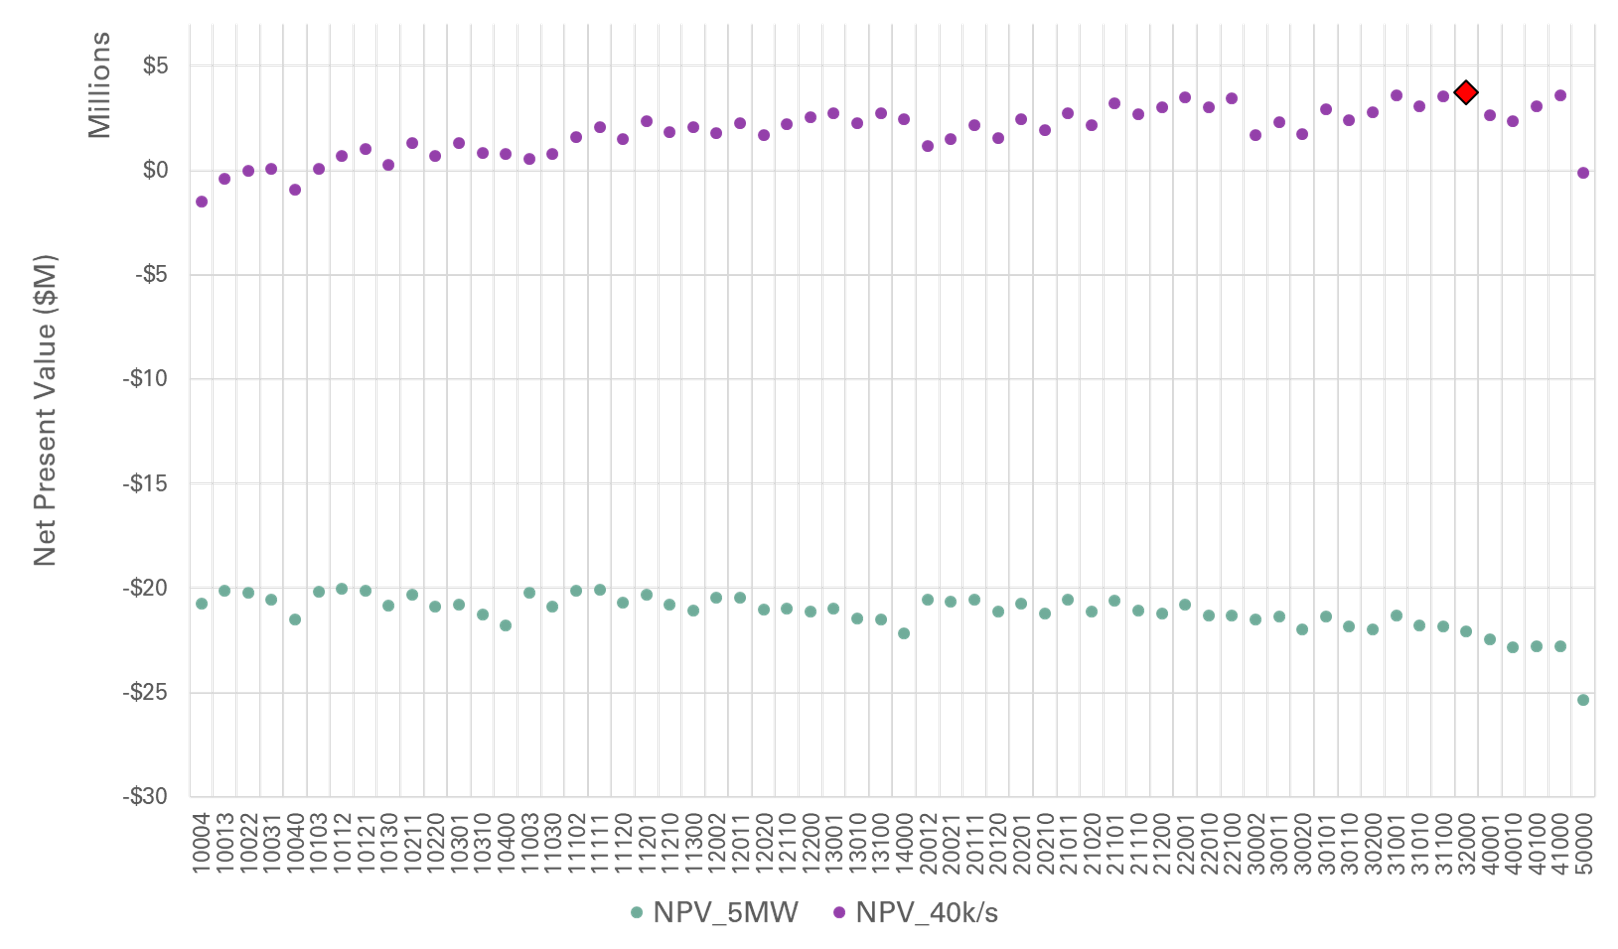
\includegraphics[width=.98\textwidth]
{templates/images/Figure-Static_Model_Construction.png}
\caption[Static cost model comparison]{Static cost model comparison between pre-set aggregate capacity (5 MW target, green) and pre-set flow rate per production well (40 kg/s, purple), plotted against module installation schedule. Both models deploy five modules in all schedule permutations involving up to a five-year period. The red diamond marks the optimal model and power plant expansion plan.}
\label{fig:static_model_compare}
\end{figure}

\subsection{Construction Optimization}
\label{ch6:static_schedule}

After lifted the fixed-capacity requirement after reviewing results in Figure \ref{fig:static_model_compare}, the hypothetical power plant modules being modeled have an predicted output of 2.1 MW based on the resource and production parameters defined in Section \ref{ch4:cm_npv}. This reduces the required module installation count to a total of three (3) modules based on the original expansion target of $\approx$5 MW. Table \ref{tab:static_optimization} revisits the installation schedule grid search exercise to determine the optimal project plan under these circumstances. At an NPV of \$1.0 million, the best option deploys two (2) modules initially and adds an additional one (1) at the end of the first year. In order to standardize cost models for direct comparison, this installation plan is used for all cost models throughout the rest of this analysis.

\begin{table}[!htp]%{R}{0.4\linewidth}
\centering
\begin{tabular}{|c|c|c|c|}
\hline
\textbf{Year 0} & \textbf{Year 1} & \textbf{Year 2} & \textbf{NPV (\$M)} \\ \hline
3 & 0 & 0 & -\$1.1 \\ \hline
1 & 0 & 2 & -\$0.3 \\ \hline
1 & 1 & 1 & \$0.5 \\ \hline
1 & 2 & 0 & \$0.6 \\ \hline
2 & 0 & 1 & \$0.6 \\ \hline
2 & 1 & 0 & \$1.0 \\ \hline
\end{tabular}
\caption[Static model module installation schedule]{Grid search for the optimal power plant installation schedule based on the static cost model. Values are in \$M, where M is million.}
\label{tab:static_optimization}
\end{table}

\subsection{Summary Statistics}
\label{ch6:static_stats}

\begin{table}[!htp]
\centering
\begin{tabular}{|l|c|}
\hline
\textbf{Static Case Statistics} & \textbf{\$M} \\ \hline
NPV & \$1.0 \\ \hline
\end{tabular}
\caption[Static model statistics]{Static model statistics. NPV is reported in \$M, where M is million.}
\label{tab:static_mod_stats}
\end{table}

\section{Probabilistic Model Metrics}

Common methods for evaluating a Monte Carlo ensemble include building a NPV histogram, constructing a \acrlong{cdf} (\acrshort{cdf} or target curve), and averaging the results together for \acrlong{enpv} (\acrshort{enpv}). Other interesting metrics for model comparison include standard deviation of NPV, extreme percentiles like P$_{05}$ and P$_{95}$, and direct comparison with the static model NPV (NPV$_{s}$). A combination of these measures is reported for each of the probabilistic model cases below.

\section{Base Case Monte Carlo}

\subsection{Model Results}
\label{ch6:base_results}

The Base Case scenario mimics the static model in form, but incorporates uncertainties in geothermal gradient, reservoir temperature, drilling \& completions costs, thermal drawdown rate, and electricity pricing to provide a more realistic range of forecasts than the deterministic cost model. No decision rules are included in this scenario. 

Results are derived from 2000 Monte Carlo realizations of the model. 

\begin{figure}[!htp]
\centering
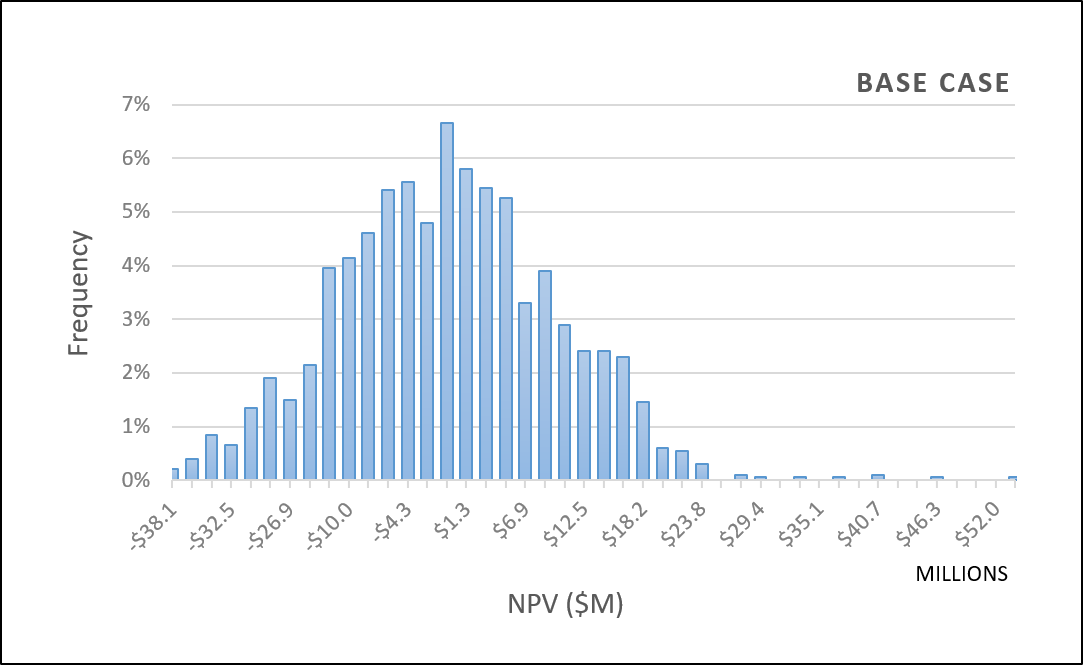
\includegraphics[width=.98\textwidth]{templates/images/Figure-Base_Case_Histogram.png}
\caption[Probabilistic Base Case histogram]{CAPTION}
\label{fig:base_case_hist}
\end{figure}

\begin{figure}[!htp]
\centering
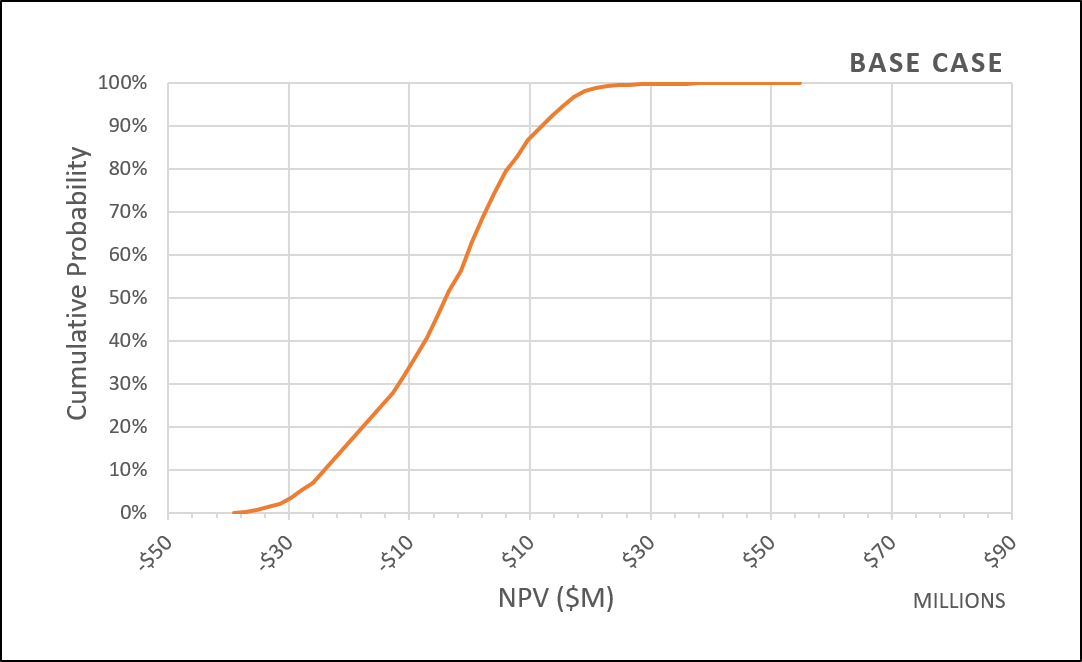
\includegraphics[width=.98\textwidth]{templates/images/Figure-Base_Case_CDF.png}
\caption[Probabilistic Base Case CDF]{CAPTION}
\label{fig:base_case_cdf}
\end{figure}

\subsection{Summary Statistics}
\label{ch6:base_stats}

\begin{table}[!htp]
\centering
\begin{tabular}{|l|r|}
\hline
\textbf{Base Case Statistics} & N=2000 \\ \hline
ENPV & -\$4.8M \\ \hline
STD(NPV) & \$13.2M \\ \hline
P05 NPV & -\$28.2M \\ \hline
P50 NPV & -\$3.9M \\ \hline
P95 NPV & \$15.9M \\ \hline
\% Difference from NPV$_{s}$ & -565\% \\ \hline
\end{tabular}
\caption[Probabilistic Base Case statistics]{Base case probabilistic model statistics for 2000 model realizations. NPV is reported in \$M, where M is million. NPV$_s$ refers to the static model NPV, as reported in Table \ref{tab:static_mod_stats}.}
\label{tab:base_stats}
\end{table}

%Results from 2000 Monte Carlo realizations are shown in Table 13. The same construction schedule highlighted in Table 12 was applied to this and all other Monte Carlo models for comparability to the deterministic case. Base Case Expected Value of NPV (ENPV) captures the average result for all realizations. At -$4.0MM, ENPV is over 200% less than NPVDet. The histogram in Figure 22 illustrates the extended tail of downside cases that drives this result. Cumulatively, ~60% of the realizations end in a net loss for the project (Figure 23). And at 2x greater than ENPV, standard deviation of NPV indicates this solution is not robust. For the deterministic case, the Flaw of Averages is in effect; by applying only the average values for uncertain variables that have a skewed probability distribution (e.g., thermal draw-down rate), the possibility of poor results is hidden from view. The Monte Carlo results display both a negative ENPV and a high likelihood of project financial loss. Without additional scenarios or clear strategies for mitigating risk, this project would and should be rejected by a responsible portfolio manager

\section{Redevelop Case Monte Carlo}

\subsection{Model Results}
\label{ch6:redevelop_results}

\begin{figure}[!htp]
\centering
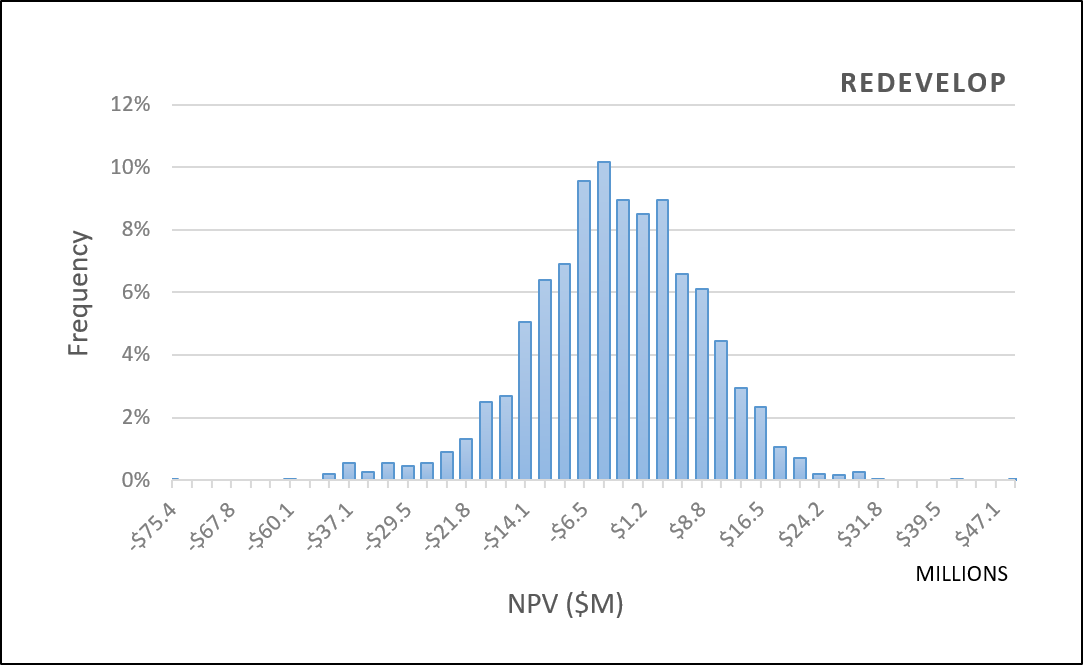
\includegraphics[width=.98\textwidth]{templates/images/Figure-Redevelop_Case_Histogram.png}
\caption[Probabilistic Redevelop Case histogram]{CAPTION}
\label{fig:redevelop_case_hist}
\end{figure}

\begin{figure}[!htp]
\centering
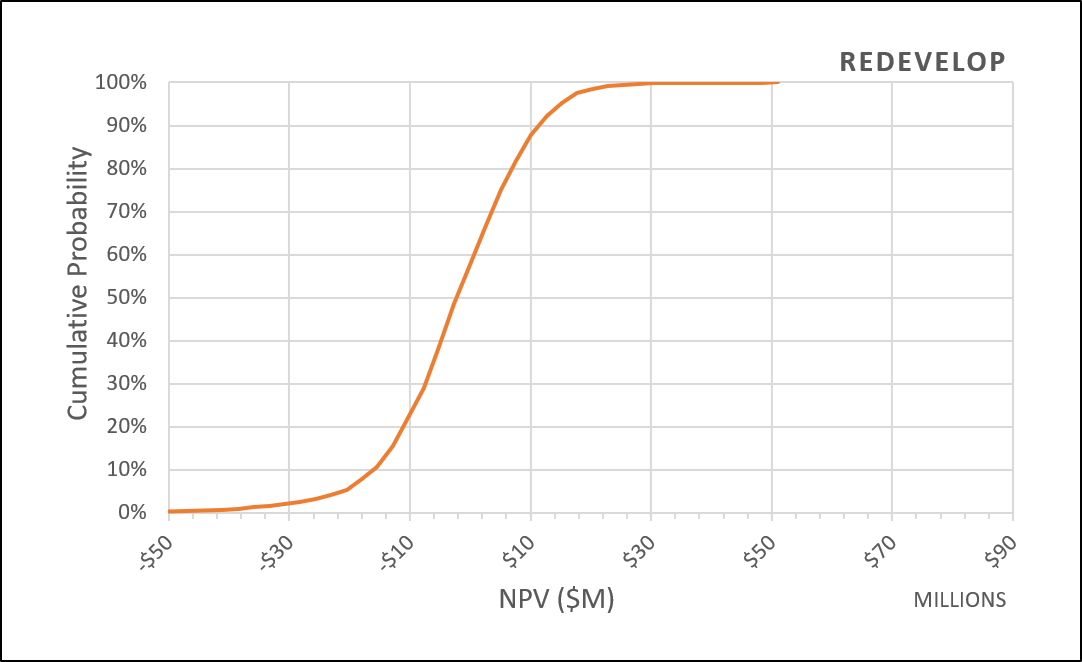
\includegraphics[width=.98\textwidth]{templates/images/Figure-Redevelop_Case_CDF.png}
\caption[Probabilistic Redevelop Case CDF]{CAPTION}
\label{fig:redevelop_case_cdf}
\end{figure}

\subsection{Summary Statistics}
\label{ch6:redevelop_stats}

\begin{table}[!htp]
\centering
\begin{tabular}{|l|r|}
\hline
\textbf{Redevelop Case Statistics} & N=2000 \\ \hline
ENPV & -\$2.5M \\ \hline
STD(NPV) & \$11.7M \\ \hline
P05 NPV & -\$21.3M \\ \hline
P50 NPV & -\$2.3M \\ \hline
P95 NPV & \$15.1M \\ \hline
\% Difference from NPV$_{s}$ & -344\% \\ \hline
\end{tabular}
\caption[Probabilistic Redevelop Case statistics]{Redevelop case probabilistic model statistics for 2000 model realizations. NPV is reported in \$M, where M is million. NPV$_s$ refers to the static model NPV, as reported in Table \ref{tab:static_mod_stats}.}
\label{tab:redevelop_stats}
\end{table}


\section{Redevelop \& Grow Case Monte Carlo}

\subsection{Model Results}
\label{ch6:grow_results}

\begin{figure}[!htp]
\centering
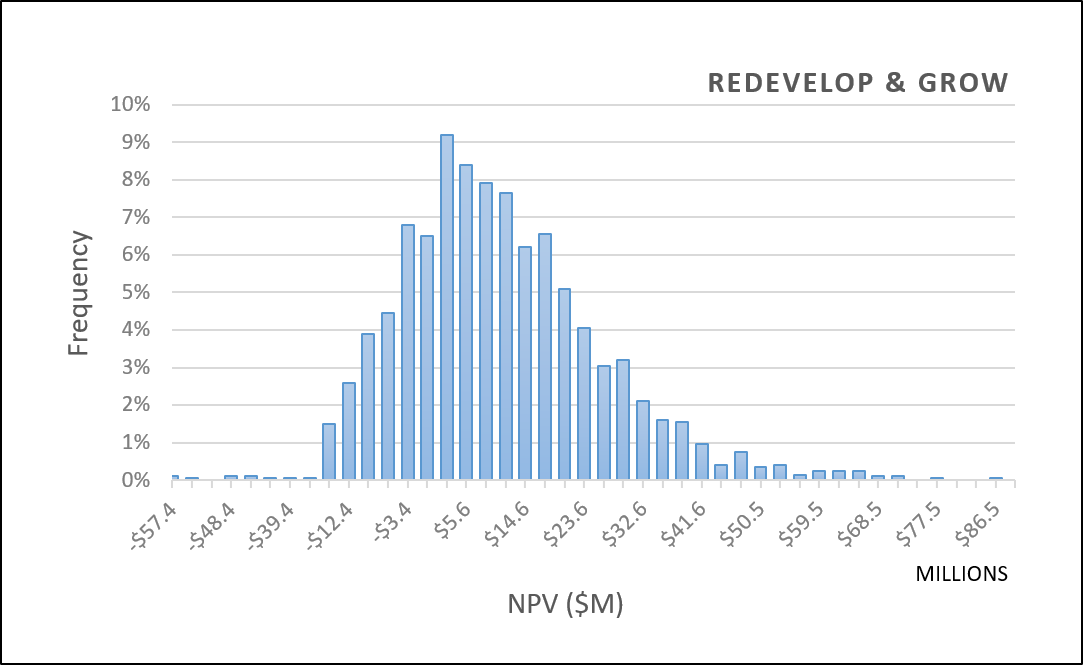
\includegraphics[width=.98\textwidth]{templates/images/Figure-Grow_Case_Histogram.png}
\caption[Redevelop \& Grow Case histogram]{CAPTION}
\label{fig:grow_case_hist}
\end{figure}

\begin{figure}[!htp]
\centering
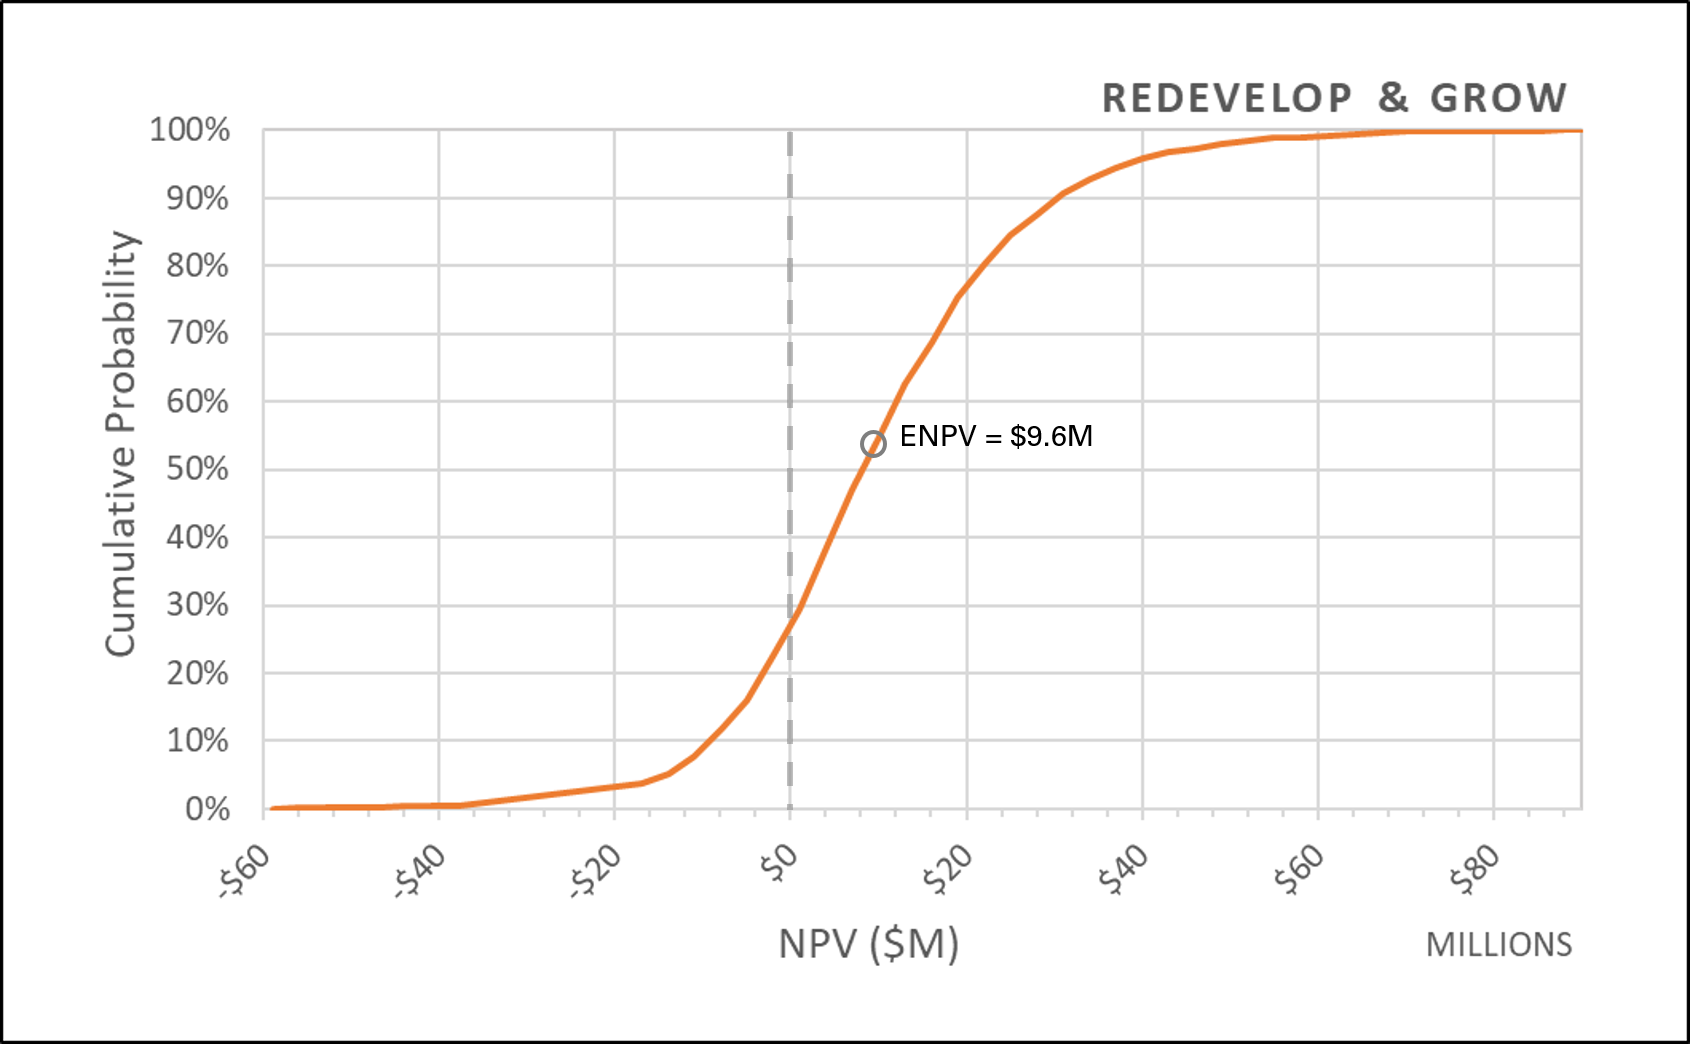
\includegraphics[width=.98\textwidth]{templates/images/Figure-Grow_Case_CDF.png}
\caption[Redevelop \& Grow Case CDF]{CAPTION}
\label{fig:grow_case_cdf}
\end{figure}

\subsection{Summary Statistics}
\label{ch6:grow_stats}

\begin{table}[!htp]
\centering
\begin{tabular}{|l|r|}
\hline
\textbf{Redevelop \& Grow Case Statistics} & N=2000 \\ \hline
ENPV & \$9.6M \\ \hline
STD(NPV) & \$16.5M \\ \hline
P05 NPV & -\$14.2M \\ \hline
P50 NPV & \$8.2M \\ \hline
P95 NPV & \$38.2M \\ \hline
\% Difference from NPV$_{s}$ & 832\% \\ \hline
\end{tabular}
\caption[Redevelop \& Grow Case statistics]{Redevelop \& Grow case model statistics for 2000 model realizations. NPV is reported in \$M, where M is million. NPV$_s$ refers to the static model NPV, as reported in Table \ref{tab:static_mod_stats}.}
\label{tab:grow_stats}
\end{table}


\section{Full Flexibility Case Monte Carlo}

\subsection{Model Results}
\label{ch6:reduce_results}

\begin{figure}[!htp]
\centering
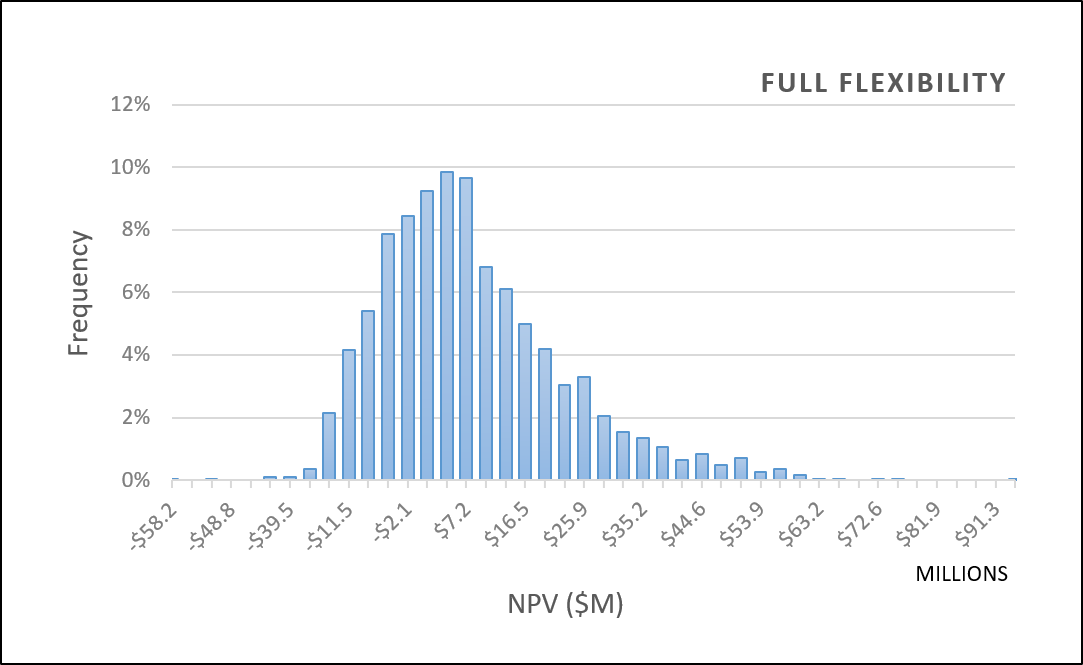
\includegraphics[width=.98\textwidth]{templates/images/Figure-Reduce_Case_Histogram.png}
\caption[Full Flexibility Case histogram]{CAPTION}
\label{fig:reduce_case_hist}
\end{figure}

\begin{figure}[!htp]
\centering
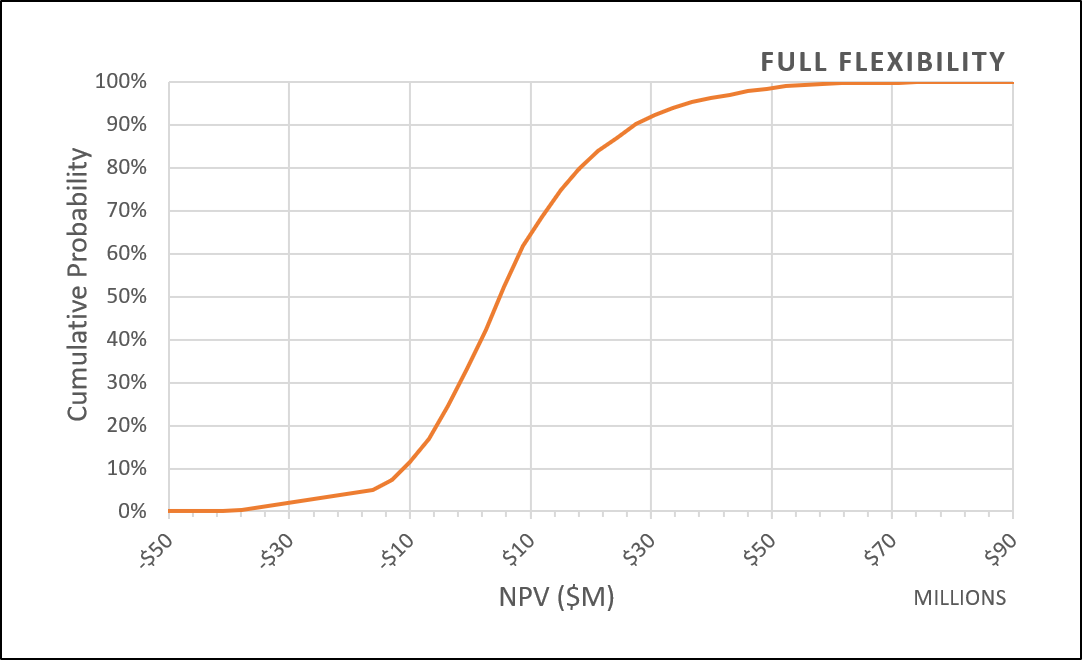
\includegraphics[width=.98\textwidth]{templates/images/Figure-Reduce_Case_CDF.png}
\caption[Full Flexibility Case CDF]{CAPTION}
\label{fig:reduce_case_cdf}
\end{figure}

\subsection{Summary Statistics}
\label{ch6:reduce_stats}

\begin{table}[!htp]
\centering
\begin{tabular}{|l|r|}
\hline
\textbf{Full Flexibility Case Statistics} & N=2000 \\ \hline
ENPV & \$6.7M \\ \hline
STD(NPV) & \$16.0M \\ \hline
P05 NPV & -\$16.3M \\ \hline
P50 NPV & \$4.9M \\ \hline
P95 NPV & \$36.2M \\ \hline
\% Difference from NPV$_{s}$ & 545\% \\ \hline
\end{tabular}
\caption[Full Flexibility Case statistics]{Full Flexibility case model statistics for 2000 model realizations. NPV is reported in \$M, where M is million. NPV$_s$ refers to the static model NPV, as reported in Table \ref{tab:static_mod_stats}.}
\label{tab:reduce_stats}
\end{table}

\section{Sensitivity}

\begin{figure}[!htp]
\centering
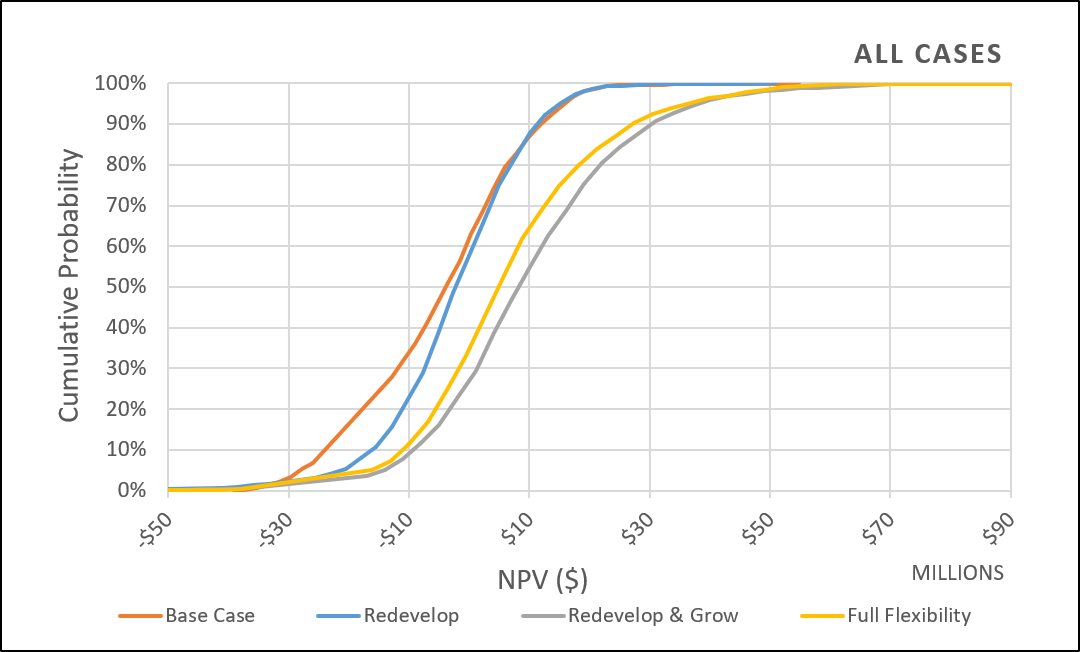
\includegraphics[width=.98\textwidth]{templates/images/Figure-All_Case_CDF.png}
\caption[All Cases CDF]{CAPTION}
\label{fig:all_case_cdf}
\end{figure}



\section{Recap}